% Fig. 3 -- OLED user-interface statechart M_UI (hierarchical extended FSM, UML state-machine notation).
% Source: firmware/esp32c3_oled_mqtt/esp32c3_oled_mqtt.ino: handleButton(), openMenuItem(),
% loopOled(), showNotice(), showMessage(), showStatus().
\documentclass[border=4pt]{standalone}
\usepackage{mathptmx}
\usepackage{amsmath}
\usepackage{tikz}
\usetikzlibrary{positioning,arrows.meta,calc,fit,backgrounds,shapes.geometric}
\begin{document}
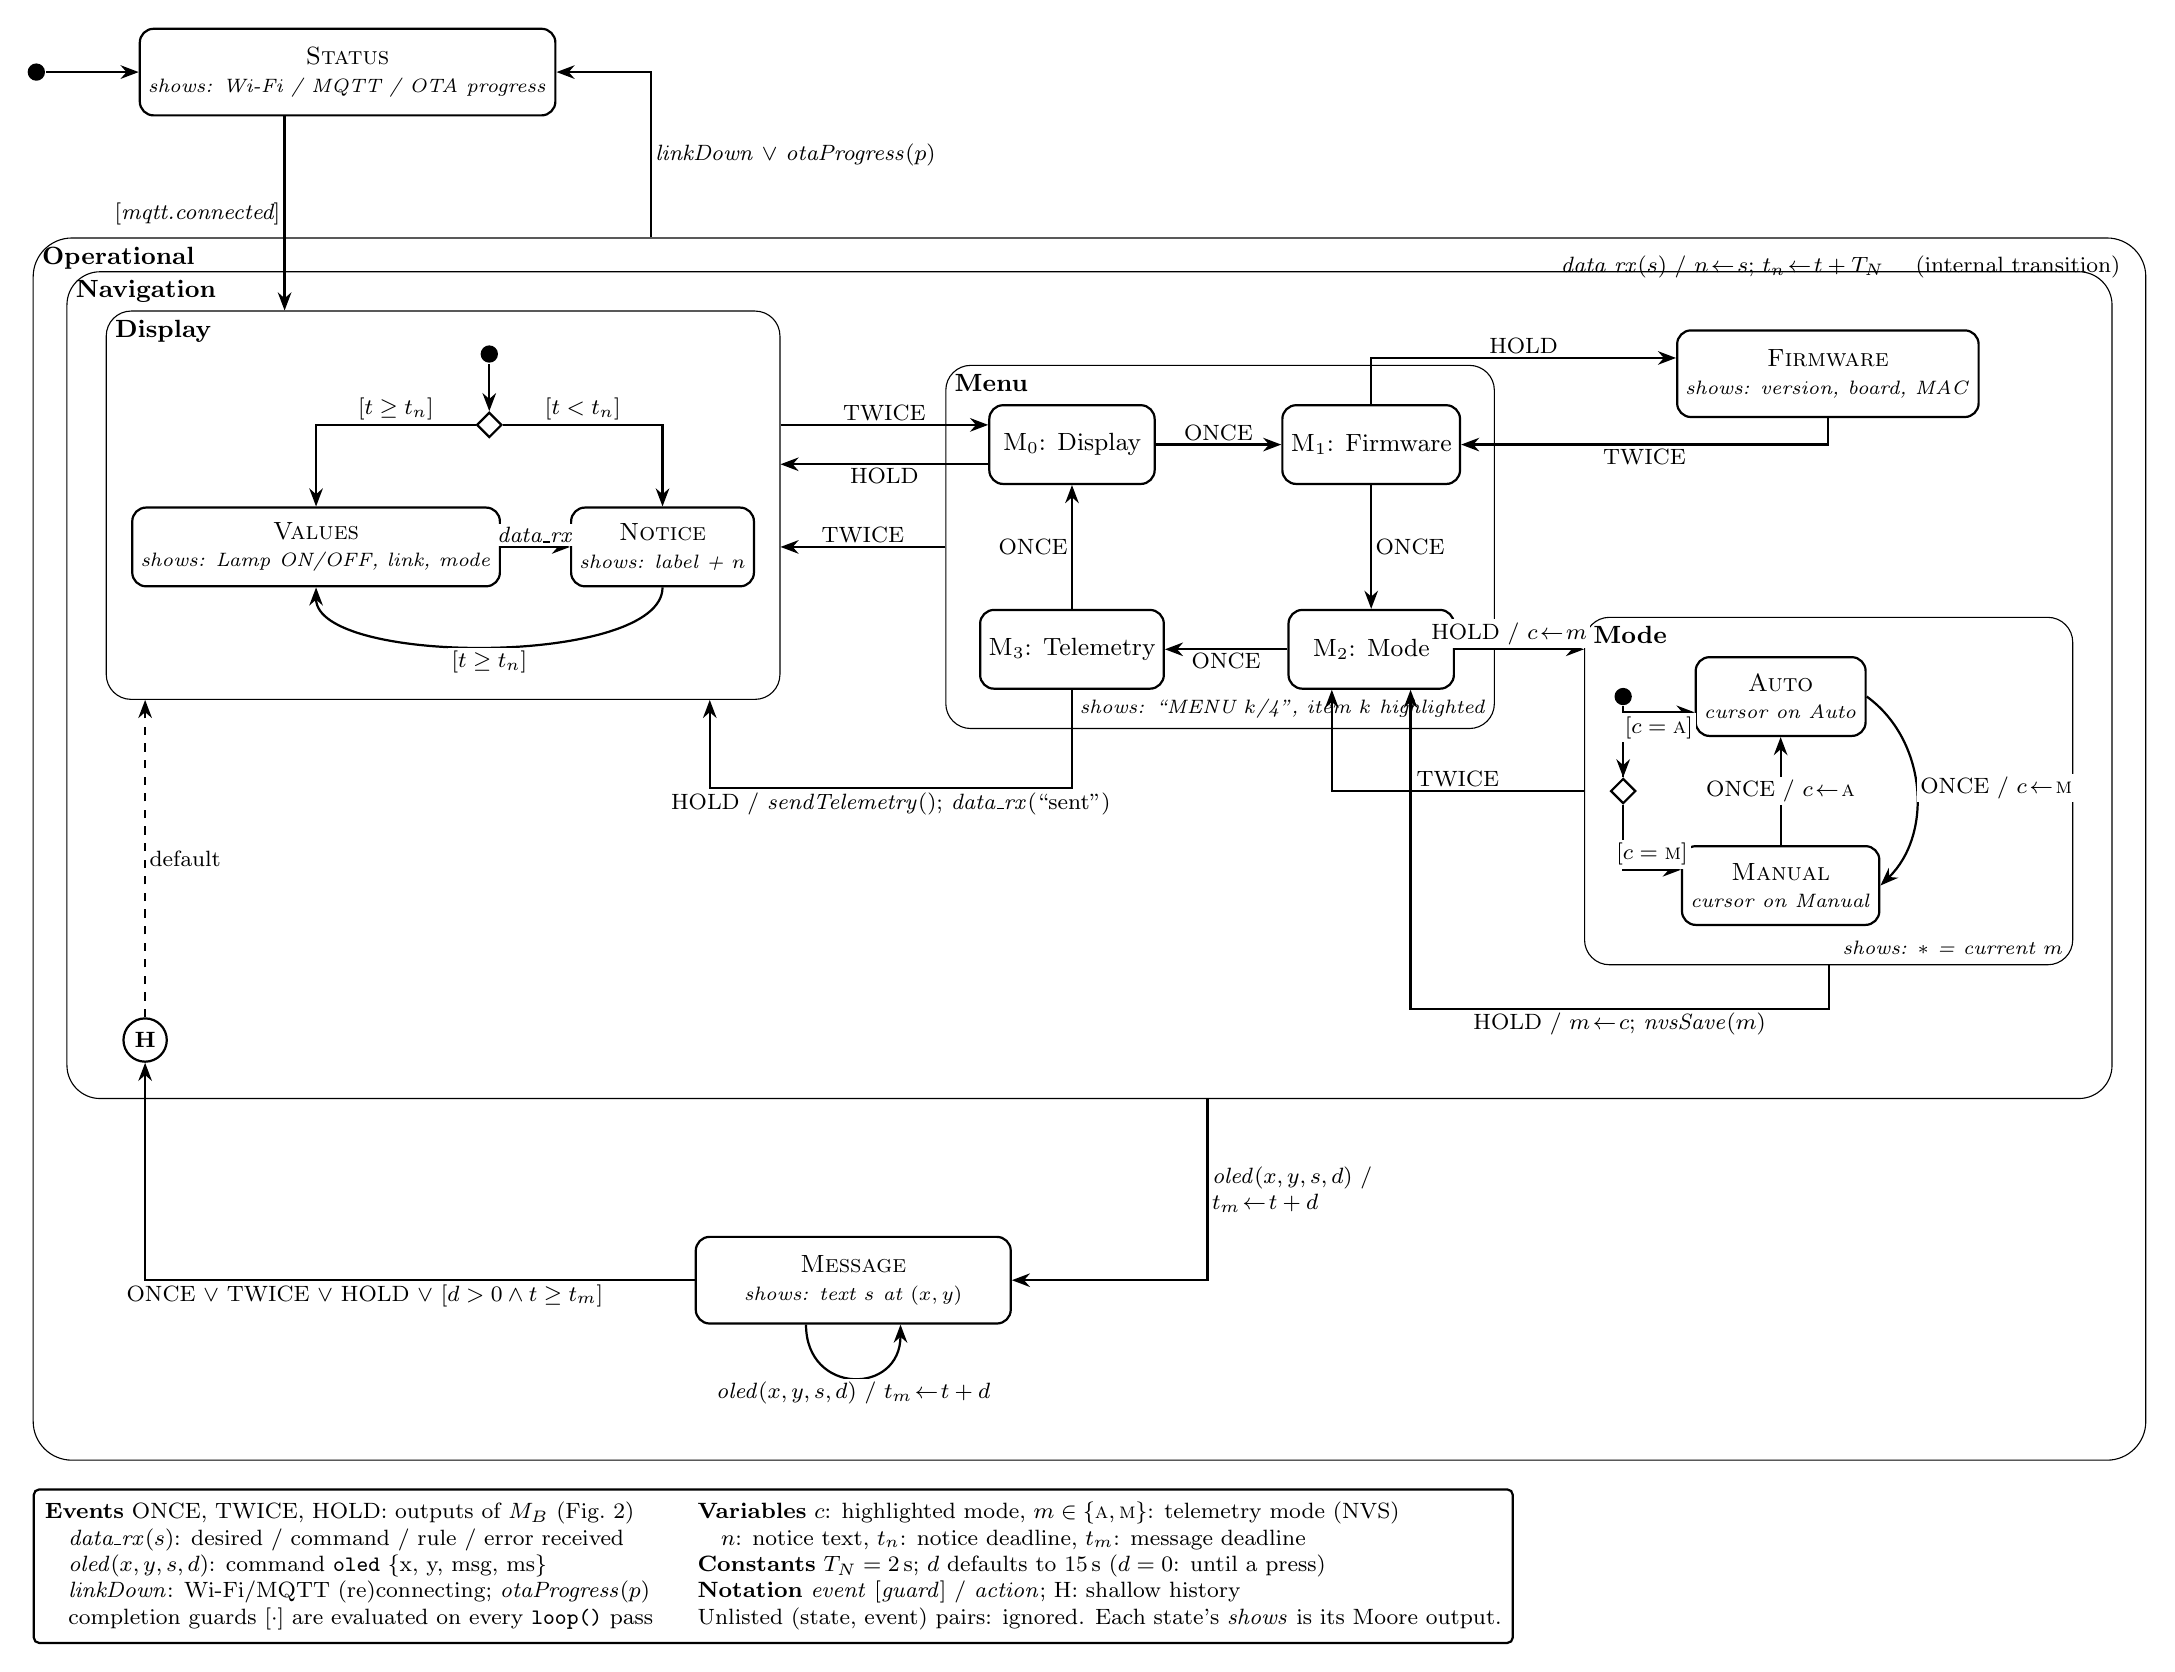
\begin{tikzpicture}[
    >={Stealth[length=2.3mm]}, thick,
    st/.style={draw, rounded corners=5pt, align=center, minimum width=24mm, minimum height=11mm,
               font=\small, inner sep=3pt, fill=white},
    sub/.style={st, minimum width=21mm, minimum height=10mm},
    comp/.style={draw, rounded corners=9pt, inner sep=9pt},
    ctitle/.style={font=\small\bfseries, anchor=north west, inner sep=3pt},
    shows/.style={font=\scriptsize\itshape},
    lab/.style={font=\footnotesize, align=center, fill=white, inner sep=1.2pt},
    init/.style={circle, fill=black, inner sep=0pt, minimum size=2.2mm},
    choice/.style={diamond, draw, inner sep=0pt, minimum size=3.2mm, fill=white},
    hist/.style={circle, draw, inner sep=0pt, minimum size=5.5mm, font=\footnotesize\bfseries, fill=white}]

  % ------------------------------------------------------------------ NAV states
  % DISPLAY (composite)
  \node[sub] (val) at (0,0)   {\textsc{Values}\\[-1pt]\textnormal{\scriptsize\itshape shows: Lamp ON/OFF, link, mode}};
  \node[sub] (not) at (4.4,0) {\textsc{Notice}\\[-1pt]\textnormal{\scriptsize\itshape shows: label + $n$}};
  \node[choice] (dch) at (2.2,1.55) {};
  \node[init] (dinit) at (2.2,2.45) {};
  \draw[->] (dinit) -- (dch);
  \draw[->] (dch) -| node[lab, pos=.25, above] {$[t \ge t_n]$} (val.north);
  \draw[->] (dch) -| node[lab, pos=.25, above] {$[t < t_n]$} (not.north);
  \draw[->] (val) -- node[lab, above] {\textit{data\_rx}} (not);
  \draw[->] (not.south) .. controls +(0,-1.0) and +(0,-1.0) .. node[lab, below] {$[t \ge t_n]$} (val.south);
  \coordinate (dlow) at ($(val.south)+(0,-1.0)$);
  \begin{scope}[on background layer]
    \node[comp, fit=(val)(not)(dinit)(dlow), inner ysep=12pt] (disp) {};
  \end{scope}
  \node[ctitle] at (disp.north west) {\textsc{Display}};

  % MENU (composite): one substate per highlighted item
  \node[sub] (m0) at (9.6,1.3)   {\textsc{M}$_0$: Display};
  \node[sub] (m1) at (13.4,1.3)  {\textsc{M}$_1$: Firmware};
  \node[sub] (m2) at (13.4,-1.3) {\textsc{M}$_2$: Mode};
  \node[sub] (m3) at (9.6,-1.3)  {\textsc{M}$_3$: Telemetry};
  \draw[->] (m0) -- node[lab, above] {ONCE} (m1);
  \draw[->] (m1) -- node[lab, right] {ONCE} (m2);
  \draw[->] (m2) -- node[lab, below] {ONCE} (m3);
  \draw[->] (m3) -- node[lab, left] {ONCE} (m0);
  \begin{scope}[on background layer]
    \node[comp, fit=(m0)(m1)(m2)(m3), inner ysep=14pt, inner xsep=12pt] (menu) {};
  \end{scope}
  \node[ctitle] at (menu.north west) {\textsc{Menu}};
  \node[shows, anchor=south east] at (menu.south east) {shows: ``MENU $k$/4'', item $k$ highlighted};

  % FIRMWARE (simple)
  \node[st] (fw) at (19.2,2.2) {\textsc{Firmware}\\[-1pt]\textnormal{\scriptsize\itshape shows: version, board, MAC}};

  % MODE (composite)
  \node[sub] (auto) at (18.6,-1.9) {\textsc{Auto}\\[-1pt]\textnormal{\scriptsize\itshape cursor on Auto}};
  \node[sub] (man)  at (18.6,-4.3) {\textsc{Manual}\\[-1pt]\textnormal{\scriptsize\itshape cursor on Manual}};
  \node[choice] (mch) at (16.6,-3.1) {};
  \node[init] (minit) at (16.6,-1.9) {};
  \draw[->] (minit) -- (mch);
  \draw[->] (mch) |- node[lab, pos=.75, below] {$[c=\textsc{a}]$} ([yshift=-2mm]auto.west);
  \draw[->] (mch) |- node[lab, pos=.75, above] {$[c=\textsc{m}]$} ([yshift=2mm]man.west);
  \draw[->] (auto.east) to[bend left=50] node[lab, right] {ONCE / $c\!\leftarrow\!\textsc{m}$} (man.east);
  \draw[->] (man.north) -- node[lab, fill=white] {ONCE / $c\!\leftarrow\!\textsc{a}$} (auto.south);
  \coordinate (moderight) at ($(auto.east)+(2.3,0)$);
  \begin{scope}[on background layer]
    \node[comp, fit=(auto)(man)(minit)(mch)(moderight), inner ysep=14pt] (mode) {};
  \end{scope}
  \node[ctitle] at (mode.north west) {\textsc{Mode}};
  \node[shows, anchor=south east] at (mode.south east) {shows: $\ast$ = current $m$};

  % ------------------------------------------------------------------ transitions between NAV states
  % Display <-> Menu: three horizontal arrows
  \draw[->] ([yshift=2.5mm]disp.east |- m0) -- node[lab, above] {TWICE} ([yshift=2.5mm]m0.west);
  \draw[->] ([yshift=-2.5mm]m0.west) -- node[lab, below] {HOLD} ([yshift=-2.5mm]disp.east |- m0);
  \draw[->] (menu.west |- val) -- node[lab, above] {TWICE} (disp.east |- val);
  % M3 --HOLD--> Display (enters Display; the choice then selects Notice)
  \draw[->] (m3.south) -- ++(0,-1.25) -| node[lab, pos=.25, below]
        {HOLD / \textit{sendTelemetry}();\ \textit{data\_rx}(``sent'')} ([xshift=6mm]not.south |- disp.south);
  % Menu <-> Firmware
  \draw[->] (m1.north) |- node[lab, pos=.75, above] {HOLD} ([yshift=2mm]fw.west);
  \draw[->] (fw.south) |- node[lab, pos=.75, below] {TWICE} (m1.east);
  % Menu <-> Mode
  \draw[->] (m2.east) -- node[lab, above, pos=.42] {HOLD / $c\!\leftarrow\!m$} (mode.west |- m2);
  \draw[->] (mode.west |- mch) -| node[lab, pos=.25, above] {TWICE} ([xshift=-5mm]m2.south);
  \draw[->] (mode.south) -- ++(0,-0.55) -| node[lab, pos=.25, below]
        {HOLD / $m\!\leftarrow\!c$;\ \textit{nvsSave}($m$)} ([xshift=5mm]m2.south);

  % ------------------------------------------------------------------ NAV superstate + history
  \coordinate (navlow) at ($(mode.south)+(0,-1.2)$);
  \begin{scope}[on background layer]
    \node[comp, fit=(disp)(menu)(fw)(mode)(navlow), inner sep=14pt, rounded corners=12pt] (nav) {};
  \end{scope}
  \node[ctitle] at (nav.north west) {\textsc{Navigation}};
  \node[hist] (h) at ($(nav.south west)+(1.0,0.75)$) {H};
  \draw[->, dashed] (h) -- node[lab, right] {default} (disp.south west -| h.north) ;

  % MESSAGE
  \node[st, minimum width=40mm] (msg) at ($(nav.south)+(-3.0,-2.3)$)
        {\textsc{Message}\\[-1pt]\textnormal{\scriptsize\itshape shows: text $s$ at $(x,y)$}};
  \draw[->] ($(nav.south)+(1.5,0)$) |- node[lab, pos=.25, right, align=left]
        {\textit{oled}$(x,y,s,d)$ /\\ $t_m\!\leftarrow\!t+d$} (msg.east);
  \draw[->] (msg.west) -| node[lab, pos=.3, below, align=center]
        {ONCE $\lor$ TWICE $\lor$ HOLD $\lor$ $[d>0 \land t \ge t_m]$} (h.south);
  \draw[->] ([xshift=-6mm]msg.south) .. controls +(0,-0.9) and +(0,-0.9) .. node[lab, below]
        {\textit{oled}$(x,y,s,d)$ / $t_m\!\leftarrow\!t+d$} ([xshift=6mm]msg.south);

  % ------------------------------------------------------------------ OPERATIONAL + STATUS
  \coordinate (oplow) at ($(msg.south)+(0,-1.3)$);
  \begin{scope}[on background layer]
    \node[comp, fit=(nav)(msg)(oplow), inner sep=12pt, rounded corners=14pt] (op) {};
  \end{scope}
  \node[ctitle] at (op.north west) {\textsc{Operational}};
  \node[font=\footnotesize, anchor=north east, align=right] at ($(op.north east)+(-0.2,-0.1)$)
        {\textit{data\_rx}$(s)$ / $n\!\leftarrow\!s$;\ $t_n\!\leftarrow\!t+T_N$ \quad (internal transition)};

  \node[st, minimum width=38mm] (stat) at ($(op.north west)+(4.0,2.1)$)
        {\textsc{Status}\\[-1pt]\textnormal{\scriptsize\itshape shows: Wi-Fi / MQTT / OTA progress}};
  \node[init] (i0) at ($(stat.west)+(-1.3,0)$) {};
  \draw[->] (i0) -- (stat);
  \draw[->] ([xshift=-8mm]stat.south) -- node[lab, left] {$[\textit{mqtt.connected}]$} ([xshift=-8mm]stat.south |- disp.north);
  \draw[->] (op.north -| stat.east) ++(1.2,0) |- node[lab, pos=.25, right, align=left]
        {\textit{linkDown} $\lor$ \textit{otaProgress}$(p)$} (stat.east);

  % ------------------------------------------------------------------ legend
  \node[draw, rounded corners=2pt, font=\footnotesize, align=left, anchor=north west, inner sep=4pt]
    at ($(op.south west)+(0,-0.35)$) {%
    \begin{tabular}{@{}l@{\hspace{16pt}}l@{}}
    \textbf{Events} ONCE, TWICE, HOLD: outputs of $M_B$ (Fig.~2) &
    \textbf{Variables} $c$: highlighted mode, $m\in\{\textsc{a},\textsc{m}\}$: telemetry mode (NVS)\\
    \quad \textit{data\_rx}$(s)$: desired / command / rule / error received &
    \quad $n$: notice text,\ $t_n$: notice deadline,\ $t_m$: message deadline\\
    \quad \textit{oled}$(x,y,s,d)$: command \texttt{oled} \{x, y, msg, ms\} &
    \textbf{Constants} $T_N = 2$\,s;\ $d$ defaults to 15\,s ($d=0$: until a press)\\
    \quad \textit{linkDown}: Wi-Fi/MQTT (re)connecting;\ \textit{otaProgress}$(p)$ &
    \textbf{Notation} \textit{event} [\textit{guard}] / \textit{action};\ H: shallow history\\
    \quad completion guards $[\cdot]$ are evaluated on every \texttt{loop()} pass &
    Unlisted (state, event) pairs: ignored. Each state's \textit{shows} is its Moore output.
    \end{tabular}};
\end{tikzpicture}
\end{document}
